% !TEX root =  MAIN.tex

\newpage

\section{Code-driven Mutation Testing: SEMuS}

\subsection{Overview}
\label{sec:semus}





To achieve \INDEX{test suite augmentation} (i.e., automatically generate test cases that kill mutants), in FAQAS, we have implemented an extension of SEMu that we call SEMu for Space Software (\INDEX{SEMuS}).

%Symbolic Execution-based Mutant analysis for Space software (FAQAS-SEMuS), is an extension of SEMu that implements test generation for space software. 

% \TODO{I've extended the following paragraph; please check}

In the FAQAS context, we cannot use SEMu as it is, since it requires mutants to be compiled with the \INDEX{LLVM compiler} in LLVM-IR format. As demonstrated with our preliminary evaluation of existing mutation analysis tools, any analysis requiring compilation into LLVM format is unlikely applicable to space software because of two reasons:  (1) our case studies rely on compiler pipelines (e.g., RTEMS) that include architecture-specific optimizations that are not supported by LLVM, and (2) there is no guarantee that the compiled objects produced by LLVM are equivalent to those produced by the original compiler (e.g., memory allocation). 

To overcome the limitations above and \EMPH{apply the test generation approach of SEMu in FAQAS} we have implemented three solutions. 
First, to avoid mutants to behave differently than the original software because of LLVM specificities (case 2 above), we rely on  MASS to identify killed and live mutants, and then compile only the live mutants into LLVM-IR format. 
Second, to increase the likelihood of successfully compiling the SUT with LLVM (case 1 above),  instead of compiling the whole software, we compile only the mutated function and its dependencies, which enables the generation of unit test cases and shall be sufficient to ensure the quality of the system under test in this context (e.g., unit test cases are normally used to ensure high code coverage). Third, to enable the generation of the meta-mutants, which is necessary to apply SEMu, we have extended MASS to (1) generate, for each source file of the SUT, both a meta-mutant processed by SEMu and the mutants processed by MASS, and (2) trace each mutant, after mutation analysis, to each mutant contained into the meta-mutant. 





% \TODO{Please add an example of a meta-mutant and single mutants generated by MASS; also, add an sentence above to refer to such listings}





Figure~\ref{fig:semus_architecture} shows the architecture of SEMuS and how it interacts with MASS. SEMuS consists of five components, which are \INDEX{Test Template Generator},  \INDEX{Pre-SEMu},  \INDEX{KLEE-SEMu},  \INDEX{KTest to Unit Test}, and \INDEX{LLVM}.
They are detailed in the following paragraphs.

\begin{figure}[h]
\begin{center}
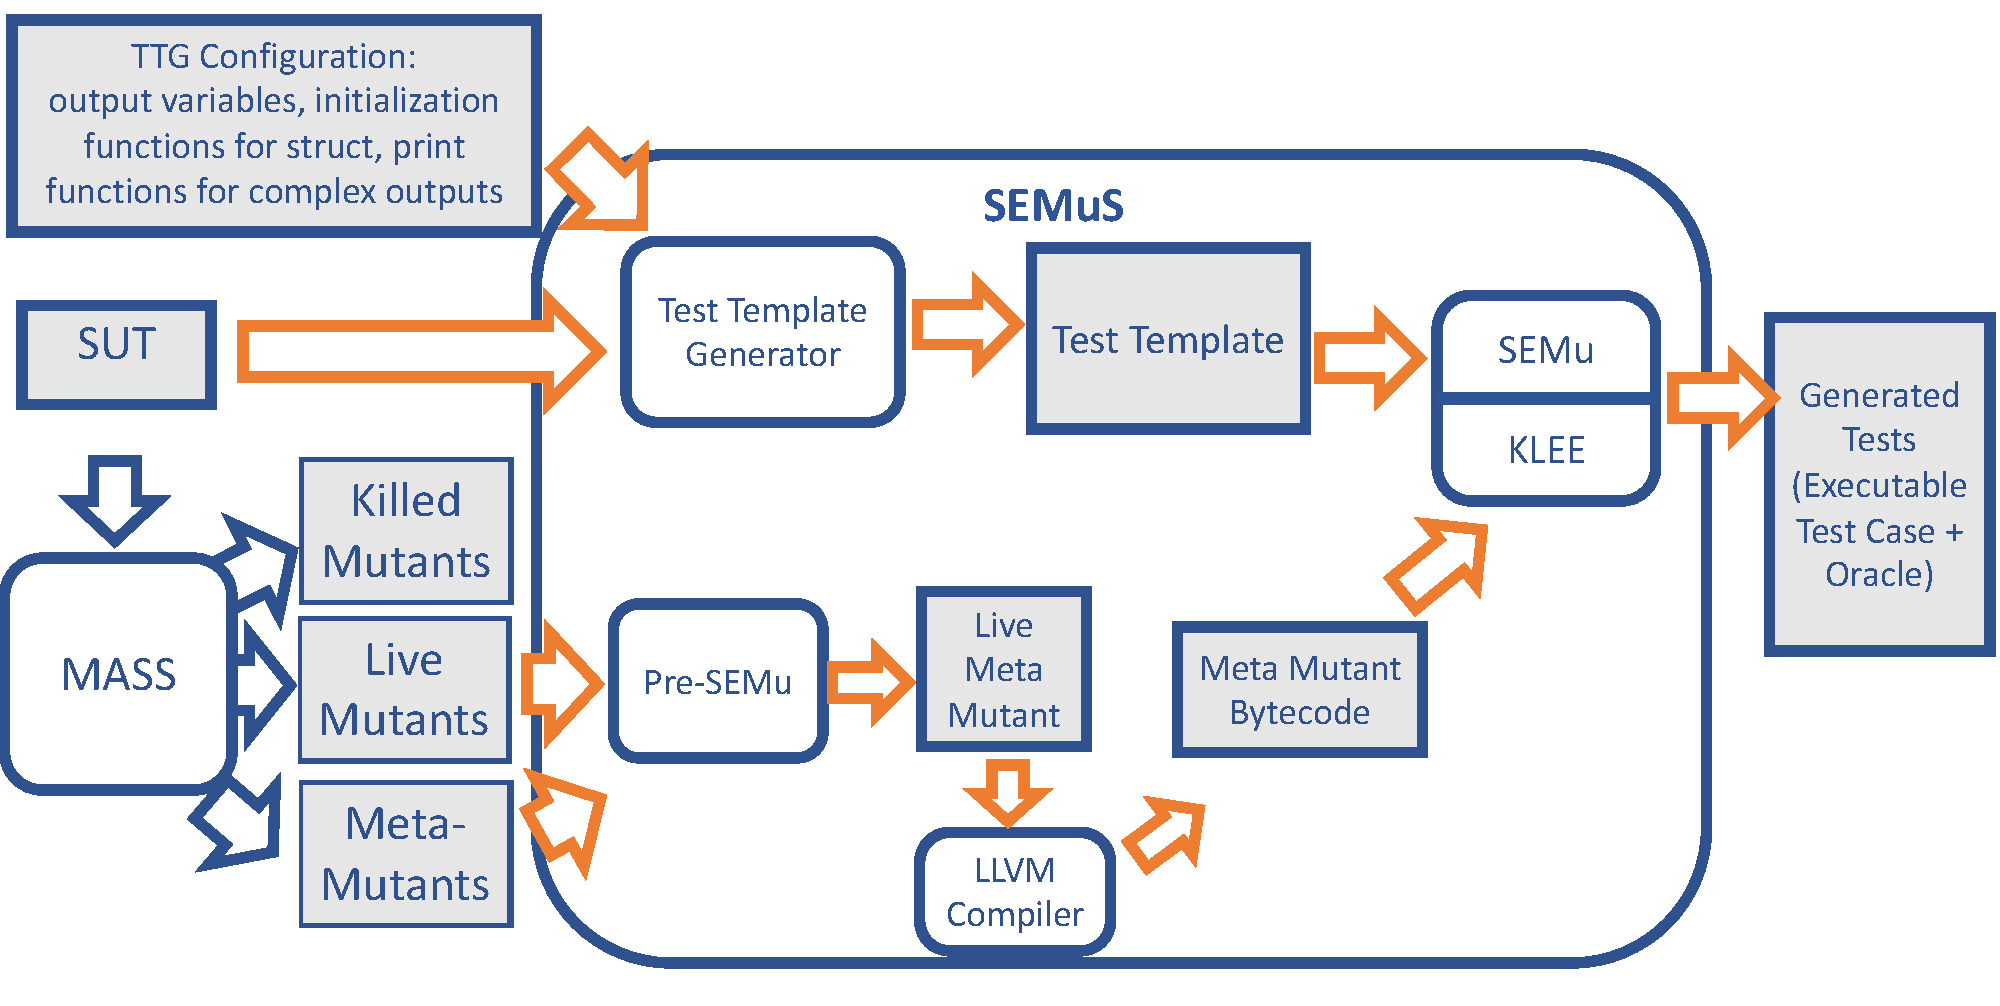
\includegraphics[width=0.8\textwidth]{images/semus-architecture2}
\caption{FAQAS-SEMuS Architecture and Workflow}
\label{fig:semus_architecture}
\end{center}
\end{figure}

%enable the adoption of SEMu in the space context. In particular, SEMuS (1) automates the generation of a test template including symbolic variables that guides the generation of test inputs, and (2) compiles the test template and the mutant into the format required by SEMu (i.e., LLVM-IR). 

\subsection{Test Template Generator}

The \INDEX{Test Template Generator} (TTG) component automates the generation of templates for the symbolic execution search. The component receives as inputs the SUT source code and the list of SUT functions. 

Listing~\ref{test_template} shows an example of a test template generated by the TTG. The TTG generates a template for every SUT function. The TTG parses the function arguments and declares them symbolic through use of the KLEE function \texttt{klee\_make\_symbolic}. Then, it adds a call to the function under analysis with symbolic values, and it saves the return value into a support variable (i.e., \texttt{result\_faqas\_semu} in Listing~\ref{test_template}). Finally, it generates a number of invocations of the \emph{printf} function that print the value of the software outputs and adds a return statement with the value returned by the function under test (e.g., \texttt{result\_faqas\_semu} in Listing~\ref{test_template}). 
Such \emph{printf} invocations are necessary because of the way SEMu determines that a mutant is killed; two are the cases in which the mutant is considered killed: (1) the main function returns a different return value, (2) different values are printed to the standard output. Consequently, it is necessary to print out all the values of the software outputs.
To select which variables to print, for every source file under test, the engineer can specify, in the SEMuS configuration file, the arguments (typically pointers) that should be either considered output or considered both input and outputs. By default, the TTG considers all the function arguments as inputs, in case some argument (e.g., a pointer to a memory buffer) is used both as input and as output the engineer shall specify it as such; similarly, in case some some argument (e.g., a pointer to a struct) is used to store outputs, the engineer shall indicate that it is an output. Moreover, since, in  the C language, the function \emph{printf} cannot automatically determine how to print the different fields specified in a data structure (i.e., it prints only the memory address of the pointer), the engineer can also specify how to printout the different fields of a data structure.

Listing~\ref{test_config} shows an example configuration file for SEMuS. In addition to output arguments (i.e., \emph{OUT\_\-ARGS\_NAMES}), input/output arguments (i.e., \emph{IN\_OUT\_ARGS\_NAMES}), and customized printf instructions (i.e., \emph{TYPES\_TO\_PRINTCODE}), the SEMuS configuration file enables the engineer to customize the generation of the test template further. Indeed, engineers can specify input argument types that should not be treated symbolically but that shall be initialized using a specific function of the SUT (i.e., \emph{TYPE\_TO\_INITIALIZATION\-CODE}); also, engineers can specify the fields, within such types (e.g., the attributes of a struct), that shall be treated symbolically.
Moreover, since the template returns the value of the function under test, the engineer can specify how to convert the returned value to int, if necessary (see parameter \emph{TYPES\_TO\_INTCONVERT}). Finally, in case the function under test receives a pointer to an array (which is typically passed as a pointer), the engineer can specify the size of such array (see parameter \emph{ARG\_TYPE\_TO\_ITS\_POINTER\_ELEM\_NUM}); by default, SEMuS assumes that a pointer refers to a single element (i.e., it is a pointer to a variable not an array).  


% !TEX root =  ../MAIN.tex

\begin{lstlisting}[style=CStyle, caption=SEMuS test template., label=test_template]
int main(int argc, char** argv) {
    // Declare variable to hold function returned value
    _Bool result_faqas_semu; 
    // Declare arguments and make input ones symbolic
    unsigned long pVal;
    int pErrCode;
    klee_make_symbolic(&pVal, sizeof(pVal), "pVal"); // Call function under test
    result_faqas_semu = T_INT_IsConstraintValid(&pVal, &pErrCode); // Make some output
    printf("FAQAS-SEMU-TEST_OUTPUT: %d\n", pErrCode);
    printf("FAQAS-SEMU-TEST_OUTPUT: %d\n", result_faqas_semu);
    return (int)result_faqas_semu;
}

\end{lstlisting}


\begin{lstlisting}[language={}, caption=Klee-test output, label=ktest]
ktest file : 'test000001.ktest'
args       : ['/MakeSym-TestGen-Input/direct/T_INT_IsConstraintValid/test.MetaMu.bc']
num objects: 2
object    0: name: b'model_version'
object    0: size: 4
object    0: data: b'\x01\x00\x00\x00'
object    1: name: b'pVal'
object    1: size: 8
object    1: data: b'\x00\x00\x00\x00\x00\x00\x00\x00'
\end{lstlisting}

% !TEX root =  ../MAIN.tex

\begin{lstlisting}[float=h, style=CStyle, caption=SEMuS configuration example., label=test_config]
{
"TYPES_TO_INTCONVERT": {},
"TYPES_TO_PRINTCODE": {"gs_timestamp_t": "printf(\"FAQAS-SEMU-TEST-OUTPUT: result_faqas_semu = tv_sec: %u, tv_nsec: %u\\n\", {}.tv_sec, {}.tv_nsec);"},
"OUT_ARGS_NAMES": ["pErrCode"],
"IN_OUT_ARGS_NAMES": ["base"],
"TYPE_TO_INITIALIZATIONCODE": {},
"TYPE_TO_SYMBOLIC_FIELDS_ACCESS": {},
"VOID_ARG_SUBSTITUTE_TYPE": "",
"ARG_TYPE_TO_ITS_POINTER_ELEM_NUM": {"char *": 6}
}
\end{lstlisting}


\subsection{Pre-SEMu}

The \INDEX{Pre-SEMu} component generates \INDEX{mutant schemata}; specifically, the component includes and compiles all the live mutants (i.e., MASS output) into a single bytecode file named the \emph{Meta Mutant}. SEMu will select which mutant to consider for test generation based on a parameter. The compilation of the Meta Mutant into LLVM bitcode is supported by the \emph{LLVM} compiler infrastructure. 

% !TEX root =  ../MAIN.tex



\begin{lstlisting}[style=CStyle, float=h, caption=Function T\_INT\_IsConstraintValid., label=original_meta]
flag T_INT_IsConstraintValid(const T_INT* pVal, int* pErrCode)
{
    flag ret = TRUE;
    (void)pVal;

    ret = ((*(pVal)) <= 50UL);
    *pErrCode = ret ? 0 :  ERR_T_INT;

    return ret;
}
\end{lstlisting}

\begin{lstlisting}[style=CStyle, float=h, caption=Mutant 1 of function T\_INT\_IsConstraintValid., label=meta_mutant_1]
flag T_INT_IsConstraintValid(const T_INT* pVal, int* pErrCode)
{
    flag ret = TRUE;
    (void)pVal;

    ret = ((*(pVal)) <= 50UL);
    *pErrCode = ret ? 1 :  ERR_T_INT;

    return ret;
}
\end{lstlisting}

\begin{lstlisting}[style=CStyle, float=h, caption=Mutant 2 of function T\_INT\_IsConstraintValid., label=meta_mutant_2]
flag T_INT_IsConstraintValid(const T_INT* pVal, int* pErrCode)
{
    flag ret = TRUE;
    (void)pVal;

    ret = ((*(pVal)) <= 50UL);
    *pErrCode = ret ? (-1) :  ERR_T_INT;

    return ret;
}
\end{lstlisting}

\begin{lstlisting}[style=CStyle, float=h, caption=Meta-Mutant for function T\_INT\_IsConstraintValid., label=meta_mutant_example]
flag T_INT_IsConstraintValid(const T_INT* pVal, int* pErrCode)
{
    flag ret = TRUE;
    (void)pVal;

    ret = ((*(pVal)) <= 50UL);

    klee_semu_GenMu_Mutant_ID_Selector_Func(1,2);
    *pErrCode = ret ? 
    	( klee_semu_GenMu_Mutant_ID_Selector==2 ?
    		((-1)):
		    (klee_semu_GenMu_Mutant_ID_Selector==1?
			    (1):
			    (0))) 
			    :  ERR_T_INT;
    klee_semu_GenMu_Post_Mutation_Point_Func(0,0);
    klee_semu_GenMu_Post_Mutation_Point_Func(1,2);

    return ret;
}
\end{lstlisting}

Listings~\ref{original_meta} provides the source code of function \emph{T\_INT\_IsConstraintValid}, while Listings~\ref{meta_mutant_1} and~\ref{meta_mutant_2} provide two example mutants generated by MASS.
Listing~\ref{meta_mutant_example} provides an example \INDEX{meta-mutant} including the same two mutants of Listings~\ref{meta_mutant_1} and~\ref{meta_mutant_2}. 
To select the mutants to analyze at runtime, SEMu relies on three support functions that shall be invoked within the eta-mutant:

\begin{itemize}
	\item \texttt{klee\_semu\_GenMu\_Mutant\_ID\_Selector\_Func}: function that takes two mutant IDs as arguments, representing a range of mutant IDs. It specifies where a portion of code containing mutants start.
    \item \texttt{klee\_semu\_GenMu\_Mutant\_ID\_Selector}: global variable that contains the ID of the mutant to be activated durng the analysis with SEMu.
	\item \texttt{klee\_semu\_GenMu\_Post\_Mutation\_Poin\_Func}: 
	function that takes two mutant IDs as arguments, it specifies where a portion of code containing mutants ends.
	It is used by SEMu to identify the portion of the code where to compare the state of the original and the mutated program and determine if the mutation has affected the program state (i.e., the \INDEX{necessity} condition to kill a mutant). In other words, it enables SEMu to perform conservative pruning and remove the mutant states that are not infected.
\end{itemize}

In Listing~\ref{meta_mutant_example}, mutant 2 from Listing~\ref{meta_mutant_2} appears on line 11 (indeed, the value \emph{-1} is selected when the mutant ID is equal to 2). Mutant 1 from Listing~\ref{meta_mutant_1} appears on line 12 (indeed, the value \emph{1} is selected when the mutant ID is equal to 1). The original software is represented by the mutant ID zero; indeed the value \emph{0} (i.e., what appears in line 7 of the Listing~\ref{original_meta}) is selected on line 14 (i.e., when the mutant ID is neither \emph{2} nor \emph{1}).

\subsection{KLEE-SEMu}



\INDEX{KLEE-SEMu} is the underlying test generation component, previously described in Section~\ref{sec:testGen:CP}. This component receives as inputs the \emph{LLVM bitcode} of the \emph{Meta Mutant} and the \emph{Test Template} for the function under test, and proceeds to apply dynamic symbolic execution to generate test inputs to kill the mutants. The output of this component are the \emph{KLEE tests}.

% \TODO{you need to list what are "the parameters of the execution"}
A \INDEX{KLEE test} is a binary file that contains information about the execution of KLEE such as the entry point of the analysis, and the generated test inputs.


An example of a KLEE test is presented in Listing~\ref{ktest}. The field \emph{args} report the entry point of the analysis; in this case, the test generation was performed for live mutants present in the function \texttt{T\_INT\_Is\-Constraint\-Valid}, which SEMuS stores in a dedicated folder. The fields named \emph{object} provide information about the outputs generated by KLEE (e.g., the generated test inputs). 
For each object, the KLEE test provides a \emph{name} (usually the name of the symbolic variable), its \emph{size}, and the actual \emph{value} generated by KLEE through constraint solving (usually this is reported in binary form).
Objects are numbered. Object number \emph{0} reports information about the data structure used by KLEE, that is, the version of the structure. The other objects report information about the generated test inputs.
Our example shows that one value of size 8 was generated for the variable \texttt{pVal}, the data field shows the binary representation of the \texttt{pVal} variable, in this case \texttt{pVal=0}.

% !TEX root =  ../MAIN.tex
\begin{lstlisting}[float=t, language={}, caption=Klee-test output, label=ktest]
ktest file : 'test000001.ktest'
args       : ['/MakeSym-TestGen-Input/direct/T_INT_IsConstraintValid/test.MetaMu.bc']
num objects: 2
object    0: name: b'model_version'
object    0: size: 4
object    0: data: b'\x01\x00\x00\x00'
object    1: name: b'pVal'
object    1: size: 8
object    1: data: b'\x00\x00\x00\x00\x00\x00\x00\x00'
\end{lstlisting}

\subsection{KTest to Unit Test}

% !TEX root =  ../MAIN.tex

\begin{lstlisting}[float=t, style=CStyle,  caption=Generated test case, label=gen_test_case]
#include <stdio.h>
#include <string.h>

#include "asn1crt.c"
#include "asn1crt_encoding.c"
#include "asn1crt_encoding_uper.c"


int main(int argc, char** argv)
{
    (void)argc;
    (void)argv;

    // Declare variable to hold function returned value
    _Bool result_faqas_semu;

    // Declare arguments and make input ones symbolic
    unsigned long pVal;
    int pErrCode;
    memset(&pVal, 0, sizeof(pVal));
    const unsigned char pVal_faqas_semu_test_data[] = {0x00, 0x00, 0x00, 0x00, 0x00, 0x00, 0x00, 0x00};
    memcpy(&pVal, pVal_faqas_semu_test_data, sizeof(pVal)); // Unsigned val is 0

    // Call function under test
    result_faqas_semu = T_INT_IsConstraintValid(&pVal, &pErrCode);

    // Make some output
    printf("FAQAS-SEMU-TEST_OUTPUT: pErrCode = %d\n", pErrCode);
    printf("FAQAS-SEMU-TEST_OUTPUT: result_faqas_semu = %d\n", result_faqas_semu);
    return (int)result_faqas_semu;
}
\end{lstlisting}



The component \INDEX{KTest to Unit Test} (KTU) converts a KLEE test into a human readable, compilable, and executable C test case. The unit test case generated by KTU, match the test template generated by TTG except for the declaration of variables where symbolic variables are replaced with concrete variables initialized with the values stored in the KTest file.
 
Listing~\ref{gen_test_case} shows an example of a test case generated for a mutant present in the function \texttt{T\_INT\_Is\-ConstraintValid}. For instance, line 20 shows that the variable \texttt{pVal} is initially filled with zeros, then in line 21, it is filled with the value stored in the variable \texttt{pVal\_faqas\_semu\_test\_data}, which holds the binary output produced by KLEE. In line 25, the function under test is invoked with the concrete value of \texttt{pVal}. 

The test case generated by the KTU prints the function return value and the value of every variable passed by reference, using the same instructions of the test template.
KTU cannot generate test assertions because only engineers can know, based on specifications, what are the values to be expected at the end of the test case execution.
However, the generated printf invocations still play the role of an oracle for regression testing, as explained in the next sections.

\subsection{Test suite augmentation} 
\label{sec:Semus:augment}
The procedure for testing with SEMuS is shown in Figure~\ref{fig:semus:test:example}.
In Step 1, the engineer executes SEMuS, which generates an output folder for every live mutant that is killed by the generated test cases.
Every folder contains: a script (i.e., \emph{runTest.sh}) that can be used to execute the generated test case, (2) the test case itself (i.e., test1.c), and (3) a text file with extension \emph{.expected} that contains the output that is observed when executing the test case with the SUT.
In Step 2, the engineer visually inspects every file with extension \emph{.expected} to determine if the observed output matches the specifications; if not, the software is faulty and needs to be fixed. In this case mutation testing enables detecting a fault. 
After verifying all the generated files with extension \emph{.expected} the engineer can reuse the test cases generated by SEMuS for regression testing in future versions of the SUT. Basically, the output folders generated by SEMuS become part of the test suite of the SUT.

When there is a new version of the SUT (Step 3, in Figure~\ref{fig:semus:test:example}), the folder with the source code of the SUT is replaced with the new version of the SUT (this can be done automatically with version control software).
The engineer can then trigger test execution by simply re-executing all the scripts \emph{runTest.sh} generated by SEMuS.
The script \emph{runTest.sh} first executes the test case (Step 4.1), then it stores the test outputs into a text file with extension \emph{.got}, finally if compares the observed output with the output generated for the previous version. If the function under test was not modified, differences may indicate that the test case FAILED.

\begin{figure}[h]
\begin{center}
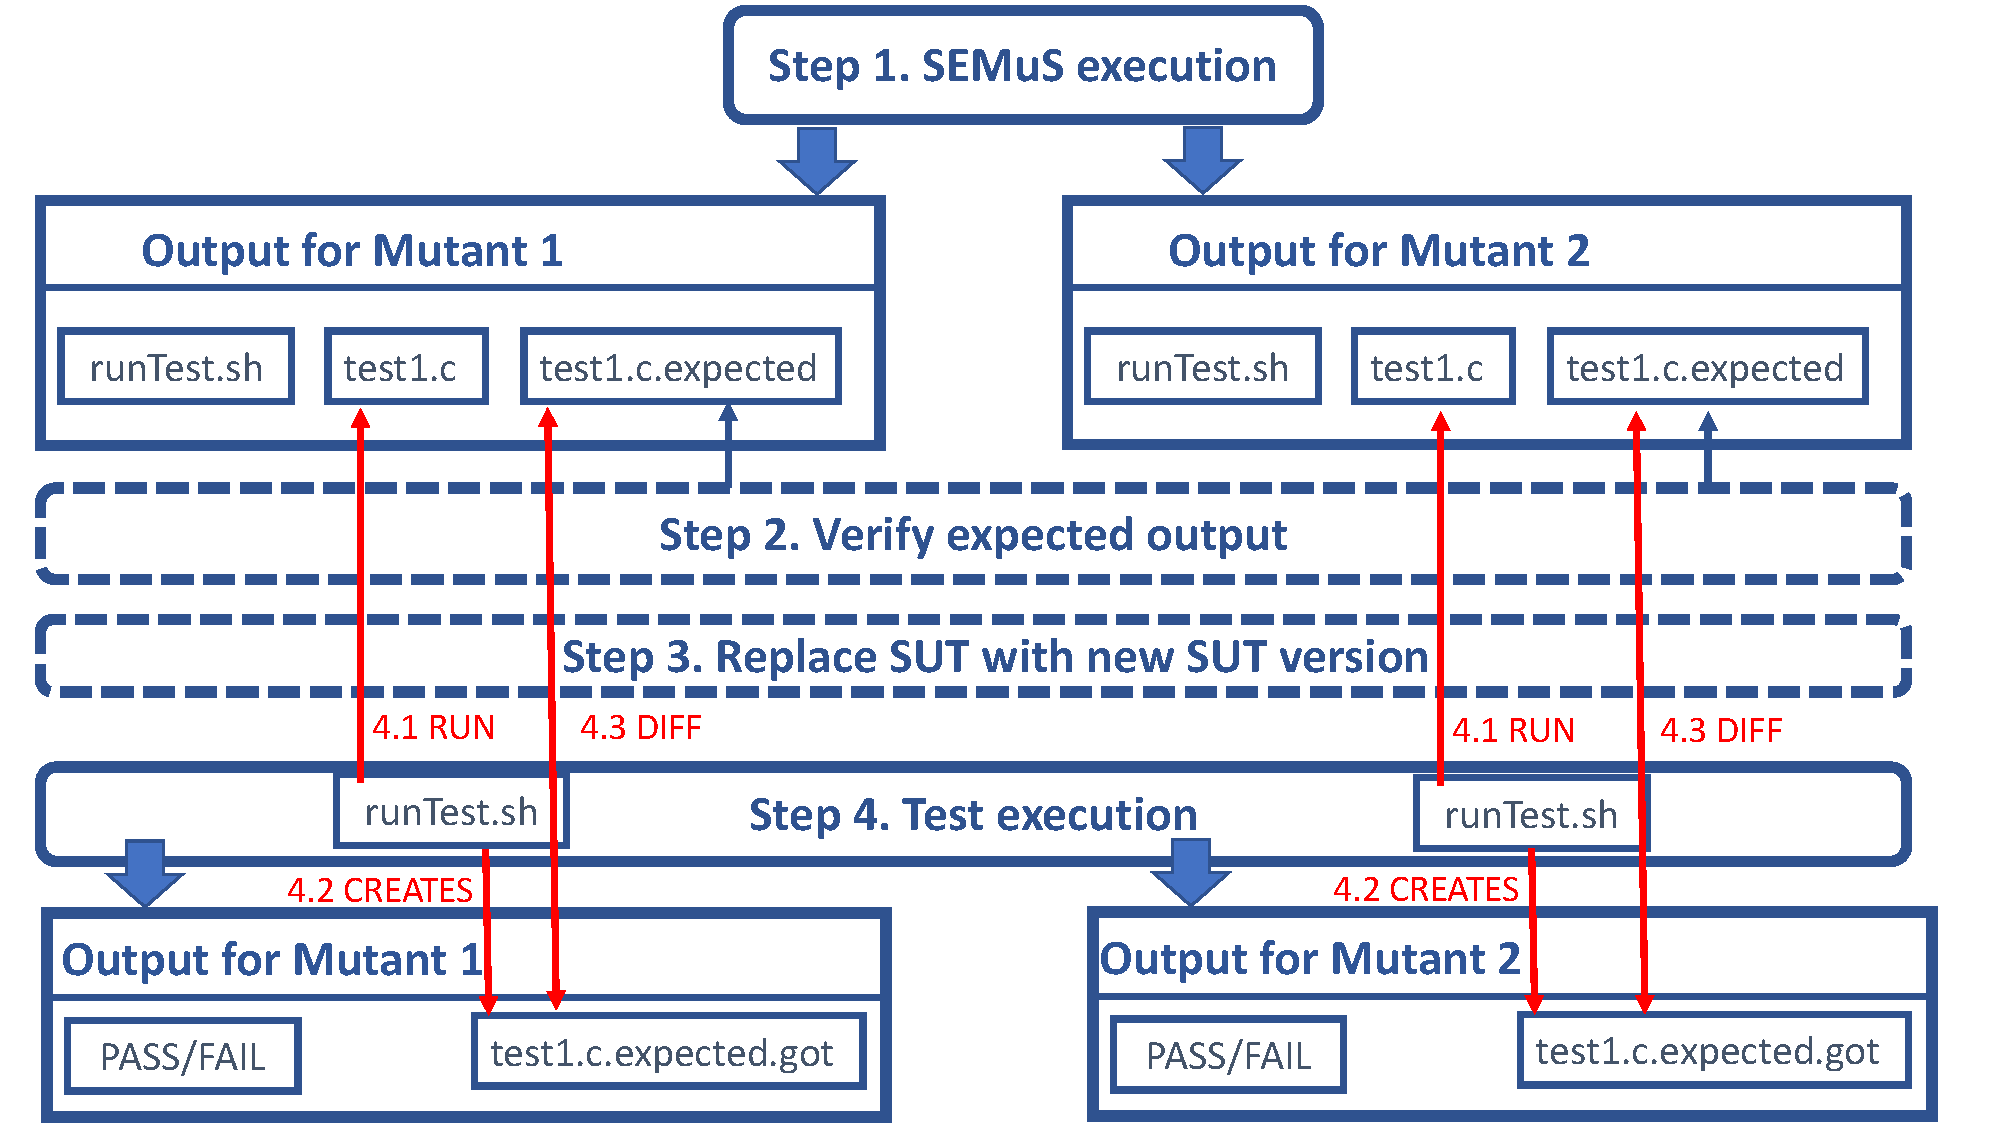
\includegraphics[width=0.8\textwidth]{images/semus-out}
\caption{Workflow for test suite augmentation with SEMuS}
\label{fig:semus:test:example}
\end{center}
\end{figure}

\subsection{Live mutants}

SEMuS may not be capable of selecting test inputs that kill the mutant under analysis. We may distinguish two cases:
\begin{itemize}
\item SEMuS execution terminates and no test case is generated.
\item SEMuS execution does terminate (i.e., it is killed after a timeout configured by the end-user, usually 15 minutes are sufficient to generate test cases).
\end{itemize}

In the first case, SEMuS has successfully exercised all the execution paths covering the mutated statements but did not identify inputs that satisfy the killing conditions. This may case indicate that the mutant is equivalent and may be discarded (however, the engineer shall verify that the test template is configured correctly). Also, we may be in such situations when some of the functions under test belong to libraries not compiled with LLVM that, consequently are not correctly processed by KLEE-SEMu; to detect these cases the engineer shall look for errors in the output generated by KLEE.

In the second case, SEMuS did not complete the analysis of the possible execution paths covering the mutated statement. Such cases may indicate that test generation is complex and probably an engineer may more efficiently select test inputs than the underlying constraint solving solution implemented by KLEE-SEMu.